\section{Path Approximation}
\label{sec:pathApprox}

 
 A natural way to approximate  $X$ (or $Y$) is to project it onto a Hilbert space. For simplicity, we focus on paths defined on the whole interval $[0,T]$, so working on $\Lambda_T$ is enough. Also, $f$ is assumed to preserve continuity, so $f(X)\in \Lambda_T$ as well.  We now  present the theory  for the original path, although the same would hold for the transformed one; see \cref{sec:funcApprox}.  
Let $\calH $ be a separable Hilbert space with inner product $(\cdot,\cdot)_{\calH}$. Then any  $X \in  \Lambda_T \cap \,  \calH $ admits the representation
\begin{equation}\label{eq:proj}
    x_t = \sum_{k} \xi_k F_k(t), \quad \xi_k = (X,F_k)_{\calH}, \quad t\in [0,T], 
\end{equation}
\vspace{-4mm}

where $\mathfrak{F} := (F_k)$ is an orthonormal basis (ONB) of $\calH$.\footnote{
The enumeration of $\mathfrak{F}$ will depend on its construction and
common notations. For instance, $\mathfrak{F}$ may or may not include an initial element $F_0$. For fairness sake, however, we always compare projections involving the same number of basis functions.} An  approximation of $X$ is obtained by truncating the  series in $\eqref{eq:proj}$, that is
$x^{K,\frakF}_t = \sum_{k\, \le\, K} \xi_k F_k(t).$ 
Each pair $(K,\frakF)$ thus induces a 
 projection map $\pi^{K,\frakF}:\calH \to \calH$ given by $\pi^{K,\frakF}(X)  = X^{K,\frakF}$. Although paths are assumed to be  one-dimensional for simplicity, the present framework is  easily generalized. Indeed, if $x_t = (x^1_t,\ldots,x^d_t) \in \R^d$,  it suffices to project each component separately, i.e. $x_t^{i,K,\frakF^i} =\sum_{k\, \le\, K} \xi^i_k F^i_k(t)$ with $\xi^i_k = (X^i,F^i_k)_{\calH}$ and $(\frakF^i)_{i=1}^{d}$ ONB's of $\calH$.
 
\subsection{Karhunen-Loève Expansion}\label{ssec:KL}
Let $\calH$ be the Lebesgue space $L^2([0,T])$ of square-integrable functions, where  we write 
$(\cdot,\cdot) = (\cdot,\cdot)_{L^2([0,T])} $ for brevity. 
Among the myriad of bases available, which one should be picked? The answer will depend upon the optimality criterion. One possibility is to minimize the square of the $L^2(\Q \otimes \, dt)-$norm (denoted by $\lVert \cdot \rVert_{*}$) between a path and its $K-$order  truncation, i.e. 
$$\epsilon^{K,\frakF} := \lVert X - X^{K,\frakF}\rVert^2_{*} = \E^{\Q} \int_0^T |
x_t - x^{K,\frakF}_t|^2 dt,$$
for $X \in \Lambda_T \cap L^2([0,T])$. 
Thanks to the orthogonality of $\frakF$,  we have 
\begin{equation}\label{eq:err}
   \epsilon^{K,\frakF} = \sum_{k,l \, > \, K}(\xi_k,\xi_l)_{L^2(\mathbb{Q})} \;(F_k,F_l)_{L^2([0,T])}  = \sum_{k \, > \, K} \lambda^{\frakF}_k , \quad \lambda^{\frakF}_k :=  \lVert  \xi_k\rVert^2_{L^2(\Q)}. 
\end{equation}
As  the mapping 
$\frakF \mapsto \sum_{k} \lambda^{\frakF}_k  $ is  constant and equal to the total variance $\lVert X\rVert^2_{L^2(\Q \otimes \, dt)}$, the projection error is solely determined by the speed of decay of  $(\lambda^{\frakF }_k)$. Inversely, the optimal basis will maximize the cumulative sum of  variance $\sum_{k \, \le \, K} \lambda^{\frakF}_k$.
This leads us to the \textit{Karhunen-Loève expansion} \cite{Karhunen,Loeve}, the continuous analogue of Principal Component Analysis. 
In what follows, assume  $\E^{\Q}[x_t]=0$ $\forall \, t \in [0,T]$ and define the symmetric kernel $\kappa_X(s,t) = (x_s, x_t)_{L^2(\Q)}.$ 
As $\kappa_X$ is also continuous and non-negative definite, Mercer's representation theorem \cite{FB/Mercer} ensures the existence of  an ONB $\frakF=(F_k)$ of $L^2([0,T])$ and scalars $\lambda_1^{\frakF} \ge \lambda_2^{\frakF} \ge \ldots \ge 0$ such that 
\begin{equation}\label{eq:mercer}
    \kappa_X(s,t)= \sum_{k=1}^{\infty} \lambda^{\frakF}_k F_k(s) F_k(t).
\end{equation}
Then $\frakF$ is the \textit{Karhunen-Loève (KL) basis} associated to $X$ under $\Q$. 
From $\eqref{eq:mercer}$, it is immediate  that   $F_k$ solves the Fredholm integral equation
 $$(\kappa_X(t,\cdot),F_k) = \lambda_k^{\frakF}\,  F_k(t), \quad  t\in [0,T].$$ Accordingly, 
 $\frakF$ and $(\lambda_k^{\frakF})$ are  termed \textit{eigenfunctions} and \textit{eigenvalues} of $\kappa_X$, respectively.  
Observe that the squared $L^2(\Q)$ norm of the KL coefficient $\xi_k=(X,F_k)$ is precisely $\lambda_k^{\frakF}$, whence comes the notation in $\eqref{eq:err}$. 
The next result reflects the relevance of the KL expansion; see \cite[Theorem 2.1.2.]{Ghanem} for a proof.

\begin{theorem}
\label{thm:KL}
The Karhunen-Loève basis
is the unique ONB of $L^2([0,T])$ minimizing $\epsilon^{K,\frakF}$  for all  $K \ge 1$. 
\end{theorem}

\begin{remark}\label{rem:center}
For non-centered trajectories,  it suffices to characterize the Karhunen-Loève basis of $x_t-\E^{\Q}[x_t]$. The projected path is then obtained by  adding the mean function back to the expansion. 
\end{remark}

\begin{example} \label{ex:KLBM} Let $T=1$ and $\Q$ be the Wiener measure, i.e. the coordinate process $X$ is Brownian motion on $[0,1]$. 
The covariance kernel is  $\kappa_X(s,t) = s \wedge t$, leading  to the eigenfunctions $F_k(t) = \sqrt{2} \sin((k-1/2)\pi t)$ and eigenvalues $\lambda_k^{\frakF} = \frac{1}{\pi^2(k-1/2)^2}$, $k \ge 1.$  
%$$F_k(t) = \sqrt{2} \sin((k-1/2)\pi t),\quad \lambda_k^{\frakF} = \frac{1}{\pi^2(k-1/2)^2}, \quad k \ge 1.$$
For $K$ large enough, the projection error is approximately equal to 
\begin{align*}
    \epsilon^{K,\frakF}
    = \frac{1}{\pi^2}\sum_{k\,>\,K} \frac{1}{(k-1/2)^2}
    \approx \frac{1}{\pi^2} \int_K^{\infty} \frac{dk}{(k-1/2)^2} = 
    \frac{1}{\pi^2(K-1/2)}.
\end{align*}
It is easily seen that $\xi_k = (X,F_k) \sim \calN(0,\lambda_k^{\frakF})$ so that $\xi_k, \xi_l$ are independent for $k\ne l$.  Therefore, "smooth" Brownian motions can be simulated  by setting
$x^{K,\frakF}_t = \sum_{k =1}^K \sqrt{\lambda_k^{\frakF}}\, z_k \, F_k(t)$ with  $(z_k)_{k=1}^K \overset{\textnormal{i.i.d.}}{\sim} \calN(0,1)$, $K\ge 1.$
\end{example}

\subsection{Lévy-Cieselski Construction}\label{ssec:LC}
Another Hilbert space  is the \textit{Cameron–Martin space}, 
$\calR = \{F \in \Lambda_T \, | \, dF \ll dt, \, \dot{F} \in L^2([0,T]) \} $ 
where $\dot{F}$ denotes the time derivative of $F$. The inner product is  $(F,G)_{\mathcal{R}} = (\dot{F}, \dot{G})$, from which 
$(F_k)$  is an ONB of  $\calR \; \Longleftrightarrow \; (\dot{F}_k)$  is an ONB of  $L^2([0,T])$
is immediate.
If $X^{K,\frakF}$ is a projected path with respect to an ONB $\frakF$ of $\calR$, then taking derivative gives
$$\dot{x}_t^{K,\frakF} = \sum_{k \, \le \, K} (\dot{X},\dot{F}_k)\dot{F}_k(t) = \sum_{k \, \le \, K} (X,F_k)_{\calR}\, \dot{F}_k(t). $$
 We gather that the projection of a path onto $\calR$ corresponds to an  $L^2([0,T])$ projection of its (possibly generalized)  derivative 
 followed by a time integration.
When $\Q$ is the Wiener measure, this procedure  is often called the \textit{Lévy-Cieselski construction}.  
With regards to accuracy, we recall the expression for the  $L^2(\Q \otimes \, dt)-$error,
$$\epsilon^{K,\frakF} = \lVert X - X^{K,\frakF}\rVert^2_{*} = \sum_{k,l \, > \, K}(\xi_k,\xi_l)_{L^2(\mathbb{Q})} \;(F_k,F_l)_{L^2([0,T])}.\vspace{-2mm}$$
As orthogonal functions in $\calR$ need not be orthogonal in $L^2([0,T])$, we cannot in general get rid of the double sum above. 
However, if $\Q$ is the Wiener measure and $\dot{X}$ the white noise process, then Fubini's theorem gives 
$$(\xi_k,\xi_l)_{L^2(\mathbb{Q})} = \int_{[0,T]^2}  \underbrace{\E^{\Q}[\dot{x}_s \dot{x}_t]}_{=\, \delta(t-s)}\dot{F}_k(s) \dot{F}_l(t) ds dt = \int_0^1 \dot{F}_k(t) \dot{F}_l(t) dt = (F_k,F_l)_{\calR}= \delta_{kl} .$$
Thus, 
$\epsilon^{K,\frakF} = \sum_{k\, >\, K} \lVert F_k \rVert^2 $.
The optimal Cameron-Martin basis would therefore have the fastest decay of its squared norms $(\lVert F_k \rVert^2)$, assuming the latter are sorted in non-increasing order.
We illustrate the Lévy-Cieselski construction with two examples, taking $T=1$.

 \begin{figure}%[H]
    \centering
     \caption{Basis functions and derivatives in the Cameron-Martin space.}
     \vspace{-2mm}
    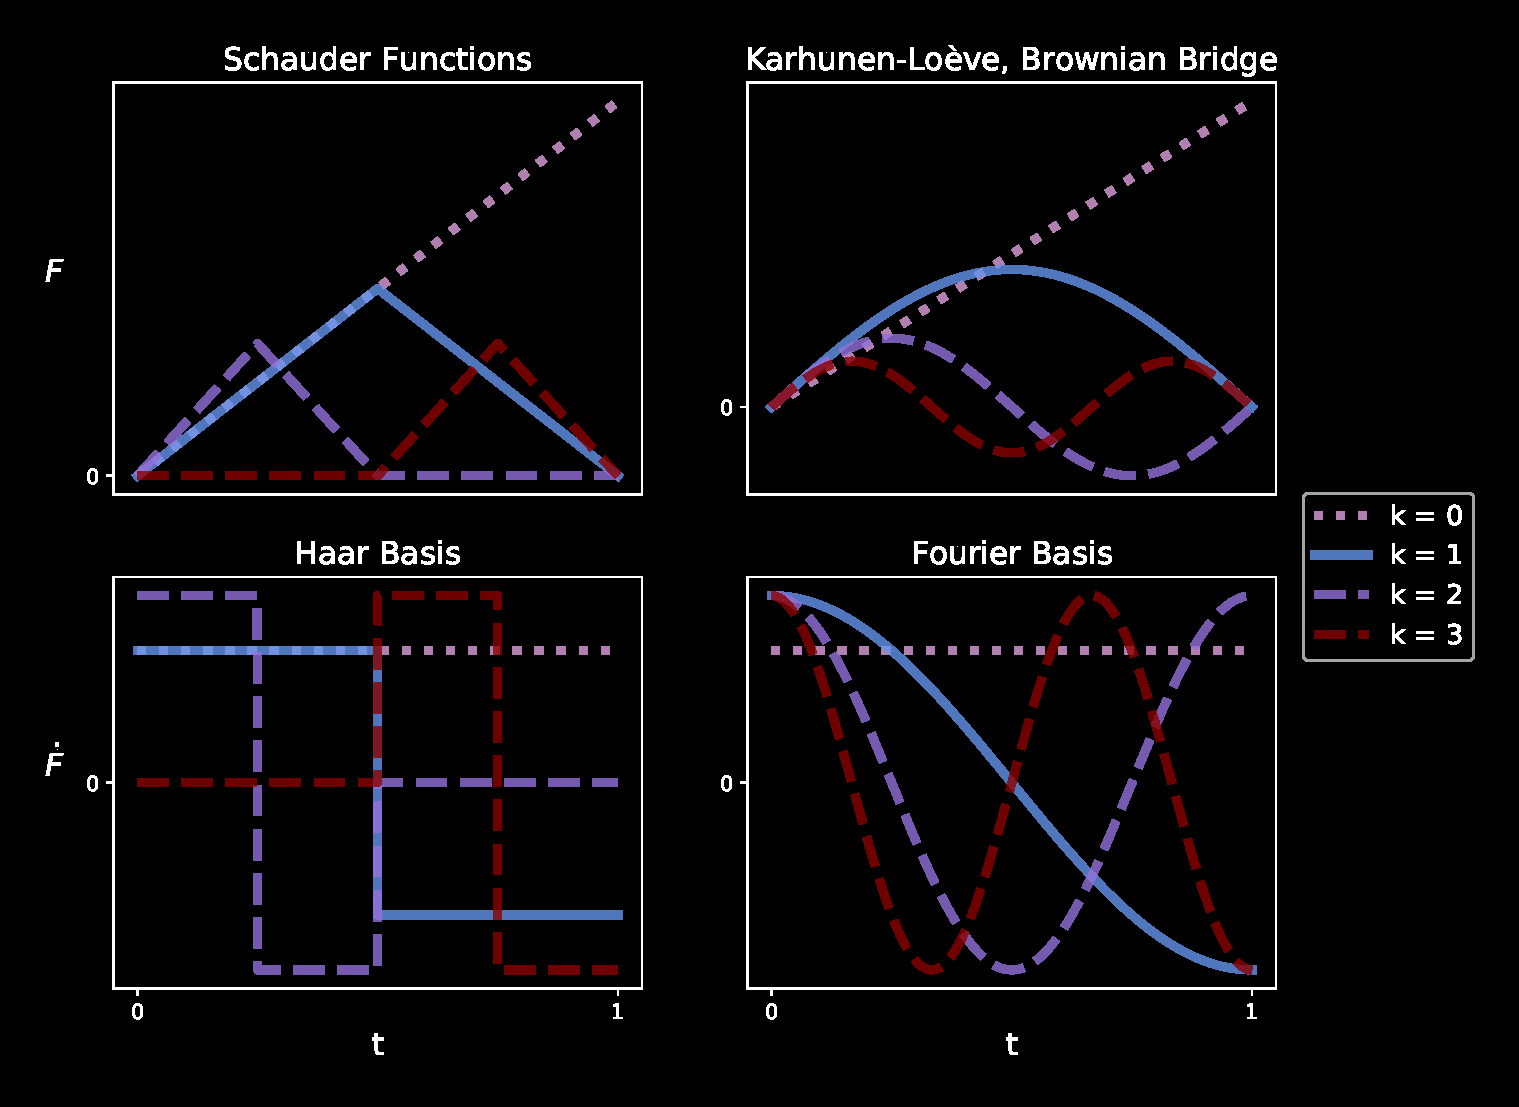
\includegraphics[scale = 0.35]{KL/Figures/LevyCieselski2.pdf}
    \label{fig:CMS}
\end{figure}

\begin{example}\label{ex:BBC}

A standard method to prove the existence of Brownian motion follows from the \text{Brownian bridge construction}. In short, it consists of a random superposition of triangular functions$-$the Schauder functions$-$obtained by integrating the Haar basis on $[0,1]$,
$$\dot{F}_{k,l}(t)=2^{k/2} \, \psi \left(2^{k}t-l\right),\quad 0 \le l \le 2^k,\quad t\in [0,1],$$
with the wavelet $\psi= (-1)^{ \mathds{1}_{[1/2, 1)}}$,  $\textnormal{supp}(\psi) = [0,1]$. It is easily seen that $\dot{F}_{k,l}$ as well as $F_{k,l}$ have support  
$[l/2^k,(l+1)/2^k]$, the $l-$th subinterval of the dyadic partition $\Pi_{k} = \{l/2^k\,|\, l = 0,\ldots,2^k\}$. 
The Schauder and Haar functions are illustrated on the left side of  \Cref{fig:CMS}.  Note that the total number of basis functions employed is $K = |\{(k,l) \,|\, 0 \le l \le 2^k , \, k=0,\ldots, \bar{K} \}| = 2^{\bar{K}+1}-1$ when considering all functions up to the $\bar{K}-$th dyadic partition. 
For Brownian motion, the approximation error is known \cite{Brown} and equal to  $\epsilon^{K,\frakF} = \frac{1}{6K}.$


\end{example}

\begin{example}\label{ex:cosine}
Let $(\dot{F})$ be the \text{cosine Fourier ONB}, i.e.
$\dot{F}_k(t) = \sqrt{2}\cos(\pi k t)$, $t \in [0,1]$. The anti-derivatives $F_k(t) = \sqrt{2}\,\frac{\sin(\pi k t)}{\pi k}$ turns out to correspond$-$up to a factor$-$to the Karhunen-Lo\`eve basis of the \text{Brownian bridge}. Indeed, recalling that $\kappa_X(s,t) = s\wedge t - st$ if $X$ is a Brownian bridge, we have for the ONB $\, \tilde{\frakF} = (\tilde{F}_k) = (\pi k \, F_k)$, 
\begin{align*}
    (\kappa_X(\cdot,t),\tilde{F}_k) 
    = \sqrt{2}\left[(1-t)\int_0^t s\, \sin(\pi k s) ds + t \int_t^1 (1-s)\sin(\pi k s) ds\right]
    = \sqrt{2}\, \frac{\sin(\pi k t)}{\pi^2 k^2},
\end{align*}
using integration by parts in the last equality. 
The eigenvalues  are therefore $(\lambda_k^{\tilde{\frakF}}) = (\frac{1}{\pi^2 k^2})$. 
The first elements of $\tilde{\frakF}$ and the Fourier cosine ONB are displayed on the right charts of  \Cref{fig:CMS}.
Following the same argument as in  \cref{ex:KLBM}, the (minimal) projection error onto $K$ basis functions is approximately equal to $\frac{1}{\pi^2 K}$. This is less than Brownian motion, as little more is known about a Brownian bridge; $\Q-$almost all trajectories return to the origin.

\end{example}

% \begin{figure}[H]
%     \centering
%     \includegraphics[scale = 0.4]{Figures/LevyCieselski.pdf}
%     \caption{Bases in the Cameron-Martin space. }
%     \label{fig:CMS}
% \end{figure}
 
 
 
 
 
 